\documentclass[a4paper]{article}
%\usepackage[cm]{fullpage}
\usepackage[utf8]{inputenc}
\usepackage[T1]{fontenc}
\usepackage{lmodern}
\usepackage[english]{babel}
\usepackage{graphicx}
%\usepackage{scrpage2}
%\usepackage{ifthen}
%\usepackage[ruled,lined]{algorithm2e}
%\usepackage{amsmath}
%\usepackage{amsthm}
%\usepackage{amssymb}
%\usepackage{units}
\usepackage{enumerate}
\usepackage{multirow}
\usepackage{fancyhdr}
\usepackage{rotating}
\usepackage{pdfpages}
\usepackage{lscape}

\begin{document}
\pagestyle{fancy}
\fancyfoot{}
\fancyhead{}
\fancyfoot[L]{SWA2011}
\fancyfoot[C]{\thepage}
\fancyfoot[R] {Group 30}
\renewcommand{\headrulewidth}{0.0pt}

\begin{center}

\includegraphics[width=1.0\textwidth]{logo}

\vspace{3cm}

\huge \textsf{\textbf{Assignment 3\\Implementation and Documentation}}

\vspace{1ex}

\Large \rm{Software Architectures}

\vspace{1ex}

\Large \rm{Summer Term 2011}

\vspace{1ex}

\normalsize Christoph Hochreiner, 0726292

\normalsize Fabian Gruber, 0726905

\normalsize Felix Rinker, 0726724

\normalsize Tobias Hochwallner, 0557189

\end{center}
\pagebreak


\tableofcontents


\pagebreak

\section{Deployment Guide}

\subsection{Prerequesits}

\paragraph{Database}
The system uses a PostgreSQL 8.4 database with the name \emph{swa} and a corresponding user with the username \emph{swa} and the password \emph{swa11}.

\paragraph{Application Server}
The prototype uses the Glassfish 3.1 application server for deploying the different components ant the Glassfish JMS implementation for the communication between these components. Therefore the $GLASSFISH\_HOME$ environment variable has to be set.

\paragraph{Build and setup the environment}
\begin{verbatim}
ant build
\end{verbatim}

The ant build target executes different tasks in order to prepare and build the prototype. These tasks cover the generation of models, creation of JMS resources and compiled the code. 

%TODO: insert single tasks that are excuted for the run task


\paragraph{Execute the prototype}
\begin{verbatim}
ant run
\end{verbatim}

The ant run target deploys the single components and the application can be accessed via \emph{http://localhost:8080/swag}.

%TODO: insert single tasks that are excuted for the build task


\section{Final Architecture}

\begin{figure}[htb]
\begin{center}
\leavevmode
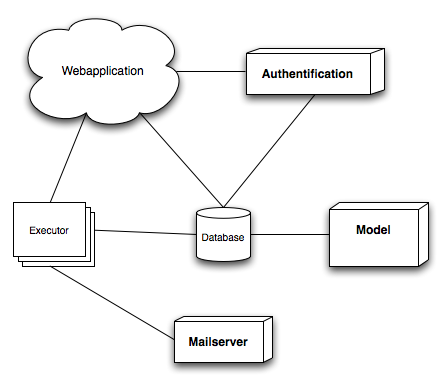
\includegraphics[width=0.8\textwidth]{Arch.png}
\end{center}
\caption{System Architecture}
\end{figure}

\begin{figure}[htb]
\begin{center}
\leavevmode
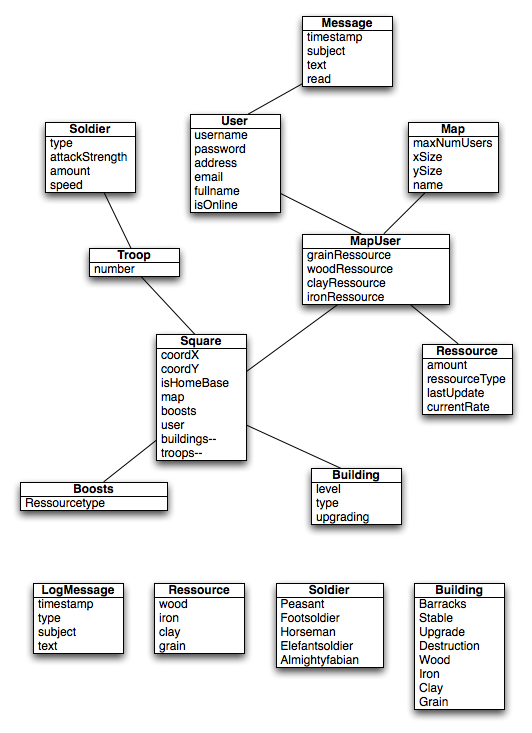
\includegraphics[width=0.8\textwidth]{Domain.png}
\end{center}
\caption{Domain model}
\end{figure}



\subsection{Components}

\subsubsection{swag-model}
This component contains the models, data access objects and data transfer objects, that were created for the second task. These classes are generated on every build process. 

\subsubsection{swag-messages}

\subsubsection{swag-util}
This sub project contains some general helper utilities for the other components. 

\subsubsection{swag-auth}

\subsubsection{swag-executor}

\subsubsection{swag-webapp}

\subsubsection{mailserver}


\subsection{Technology stack}
\paragraph{Apache Wicket}\footnote{http://wicket.apache.org/}
The Apache Wicket Framework was used for the creation of the Web application.

\paragraph{Guice}\footnote{http://code.google.com/p/google-guice/}
Guice was used for the dependency injection.

\paragraph{Quartz Scheduler} \footnote{http://www.quartz-scheduler.org/}
For the implementation of our delayed actions, we integrated the quartz scheduler, that provides the necessary functionality to schedule tasks, that are executed to specific dates in the future.

\paragraph{JMS}
The JMS technology was used for the communication between the components. For this prototype, we relied on the JMS implementation of the Glassfish Server.

\paragraph{Maven}
For development purposes we used maven in order to build, setup and deploy the applications. In order to meet the requirements, we transformed our maven targets to ant with <TODO insert Plugin>



%TODO add additional technologies

\section{Planned but omitted implementations}
Due to some implementation and particularly configuration and execution issues with the Glassfish Server, we could not implement all planed features. This chapter lists all significant omitted features.

\paragraph{advanced troop and battle management}
We have planned some handy features in the area of battles an troops. On of the features is the dedicated selection of soldiers for a specific battle. This feature  allows the user to only send selected soldiers instead of the whole troop. The second feature that has to be omitted was the planned routing component, that calculates the duration for the march for the specific soldiers, depending on the slowest one. This component would have enriched the game in order to role out special tactics to attack other players. The last component in this area is the destruction of buildings. For this feature we planned, that the attacker can use his destruction units in order to destroy hostile buildings. When all defendant soldiers are dead, the destruction units need some time, according to the amount of units, and the level of the building, to tear the building down.

\paragraph{Highscores as a webservice}
The highscores should display some ranking for users. These ranking is divided in to sections, the economic part and the military part. The economic part should cover the level of the buildings and the resources while the military part should cover the current offensive power. Due to the fact that the highscore generation requires multiple inefficient queries, this generation should only be carried out every 15 minutes. The generation should be executed on an own component and this component should provide the statistics via a WDSL connection. This connection has numerous advantages, the main advantage is the simple integration of the statistics in the web application, but also other stakeholders can implement these statistics in order to produce own advanced statistics.

\paragraph{upgrades for soldiers}
The building Upgrades in the base should provide specific upgrades for every soldier. These upgrades improve either the speed or the attack strength of the soldiers.

\paragraph{timed actions}
The most important feature would could not implement due to time issues, is the task issue component. We have planned to implement an action executor, that carries out tasks in the future, e.g. finishing a building or attacking a hostile village. Therefore the web application creates a issue at the action executor via JMS and sets a timestamp in the future to this issue. When the time has arrived, the action executor asynchronous executes the issue, updates the database and sends notifications to the users about the event. This timing should be carried out by the Quartz scheduler, that has already been implemented. This scheduler stores the issues and invokes them, when their time has come.


\section{Possible Improvements}
\paragraph{Server side caching of components of the web application}
Due to the fact that browser based games normally suffer from numerous page reloads, server side caching of single components can achieve a great leap forward concerning performance issues. Some components, like maps change only rarely and they could be cached on the server. The framework wicket provides some functionality to control the caching of components on the server. \footnote{https://cwiki.apache.org/WICKET/caching-in-wicket-15.html} This manual caching configurations can produce severe issues for the update of web components, therefor they should only be used in combination of a comprehensive test coverage of the application.

\paragraph{Caching of database queries}
Modern databases provide numerous possibilities to improve the performance of queries. Some options cover the general handling of queries, but there are also some additions functionalities e.g. views, that can cache certain records and therfore reduce the load on the database.

\paragraph{Performance Monitoring}
Numerous performance issues can only be identified during runtime. Therefore you have to implement some performance monitoring functionality. There are to different approaches for performance monitoring. The first approach is the global monitoring on the application server. This approach can only detect severe performance issues. In order to identify these issues you often have to implement some specific monitoring functionality , e.g. with JAMON. \footnote{http://jamonapi.sourceforge.net/}

\end{document}
